\section{Pipeline}\ohead{Sebastian Schmitt}
Die einzelnen Schritte der Pipline werden teilweise in unterschiedlichen Klassen implementiert.
Die \autoref{fig:pipeline-classes} gibt einen Überblick über diese sowie deren Beziehungen zueinander.

\begin{figure}
    \centering
    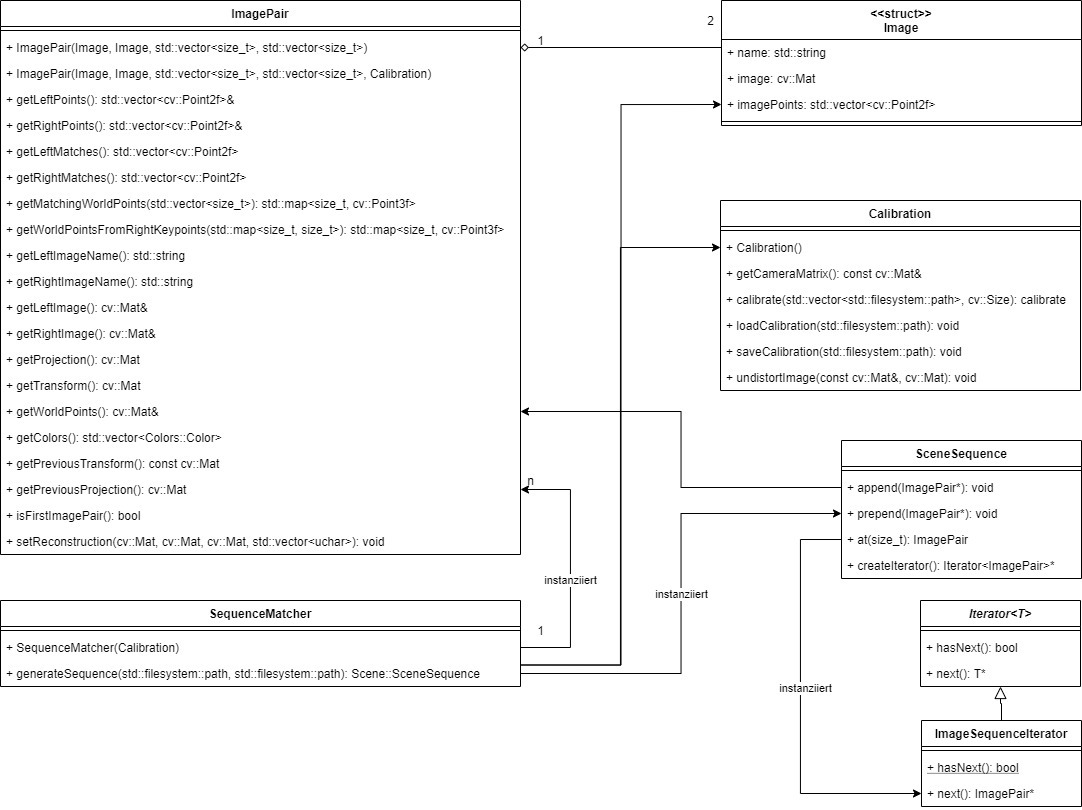
\includegraphics[width=\textwidth]{src/img/classes.jpg}
    \caption{Klassendiagramm alle Klassen welche Pipeline Funktionen implementieren}
    \label{fig:pipeline-classes}
\end{figure}